% Fig. 5 - ToA Clustering Mechanism
% Compile: pdflatex fig5_toa_clustering.tex
\documentclass[border=8pt]{standalone}
\usepackage{amsmath}
\usepackage{tikz}
\usetikzlibrary{arrows.meta, positioning, calc, decorations.pathreplacing, fit}

\begin{document}
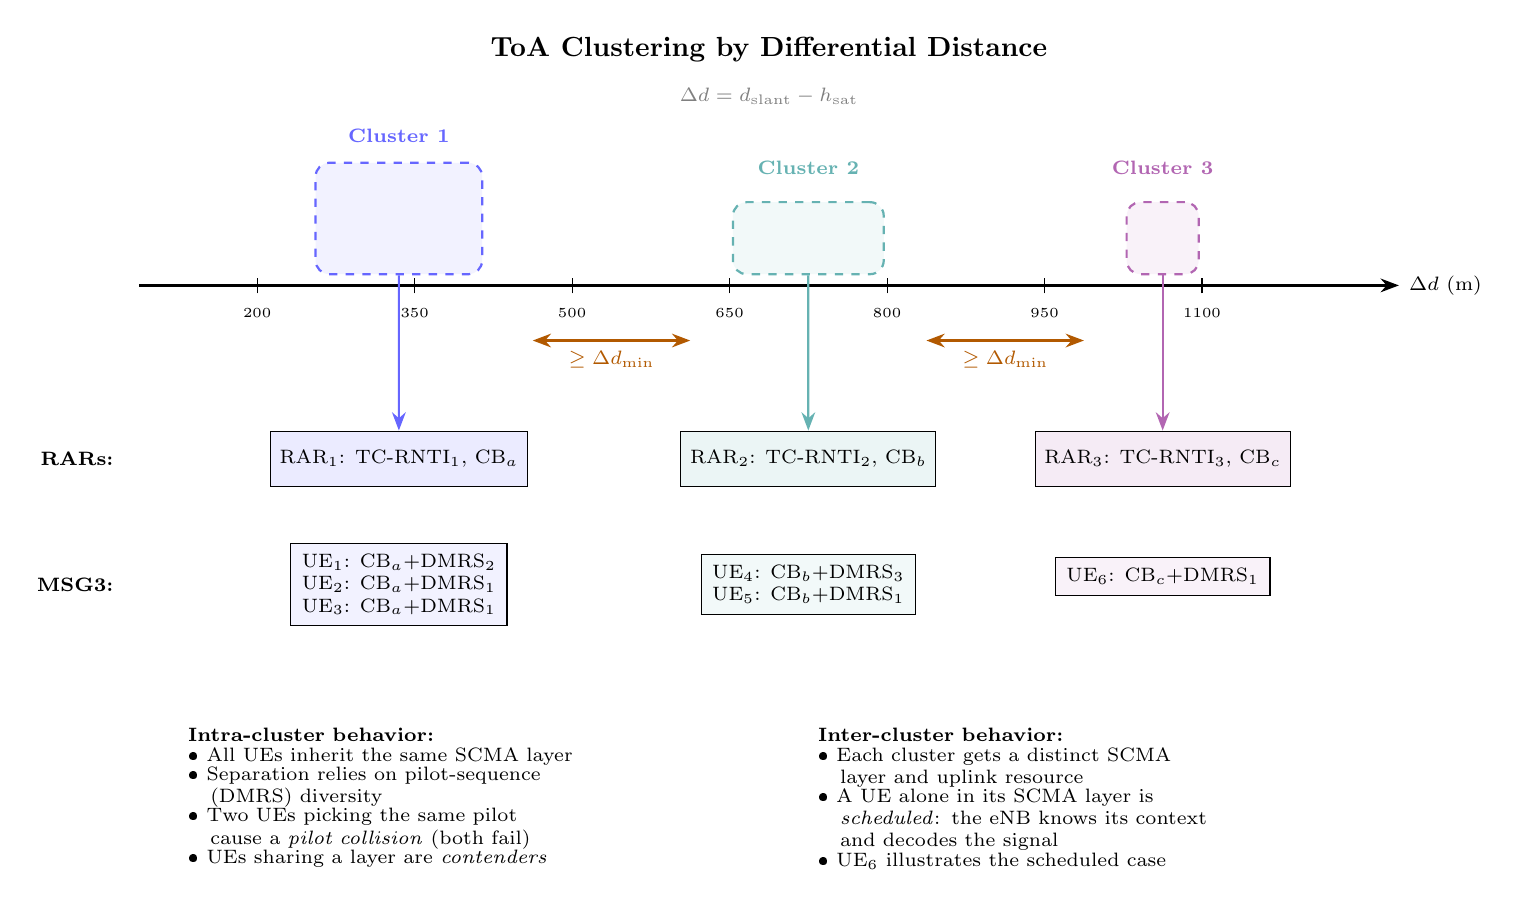
\begin{tikzpicture}[
    >=Stealth,
    font=\footnotesize,
    ue/.style={draw, circle, minimum size=0.55cm, inner sep=0pt, font=\tiny\bfseries},
]

% === Title ===
\node[font=\normalsize\bfseries] at (7.5, 3) {ToA Clustering by Differential Distance};
\node[font=\scriptsize, text=gray] at (7.5, 2.4)
     {$\Delta d = d_{\text{slant}} - h_{\text{sat}}$};

% === Axis ===
\draw[thick, ->] (-0.5, 0) -- (15.5, 0) node[right, font=\scriptsize] {$\Delta d$ (m)};

\foreach \x/\lbl in {1/200, 3/350, 5/500, 7/650, 9/800, 11/950, 13/1100} {
    \draw (\x, -0.1) -- (\x, 0.1);
    \node[font=\tiny, below=2pt] at (\x, -0.1) {\lbl};
}

% === UEs positioned on axis ===
% Cluster 1: around 300-400m (3 UEs, same codebookId)
\node[ue, fill=blue!25] (u1) at (2.2, 0.6) {1};
\node[ue, fill=blue!25] (u2) at (3.4, 0.6) {2};
\node[ue, fill=blue!25] (u3) at (2.8, 1.1) {3};

% Cluster 2: around 700-800m (2 UEs, different codebookId)
\node[ue, fill=teal!25] (u4) at (7.5, 0.6) {4};
\node[ue, fill=teal!25] (u5) at (8.5, 0.6) {5};

% Cluster 3: around 1050m (1 UE, different codebookId)
\node[ue, fill=violet!25] (u6) at (12.5, 0.6) {6};

% === Cluster boundaries ===
\node[draw=blue!60, dashed, thick, rounded corners=5pt,
      fill=blue!5, fit=(u1)(u2)(u3), inner sep=5pt] (c1) {};
\node[font=\scriptsize\bfseries, text=blue!60] at (2.8, 1.9) {Cluster 1};

\node[draw=teal!60, dashed, thick, rounded corners=5pt,
      fill=teal!5, fit=(u4)(u5), inner sep=5pt] (c2) {};
\node[font=\scriptsize\bfseries, text=teal!60] at (8, 1.5) {Cluster 2};

\node[draw=violet!60, dashed, thick, rounded corners=5pt,
      fill=violet!5, fit=(u6), inner sep=5pt] (c3) {};
\node[font=\scriptsize\bfseries, text=violet!60] at (12.5, 1.5) {Cluster 3};

% === Separation arrows ===
\draw[<->, thick, orange!70!black] (4.5, -0.7) --
     node[below, font=\scriptsize] {$\geq \Delta d_{\min}$} (6.5, -0.7);
\draw[<->, thick, orange!70!black] (9.5, -0.7) --
     node[below, font=\scriptsize] {$\geq \Delta d_{\min}$} (11.5, -0.7);

% === Resource mapping ===
\node[font=\scriptsize\bfseries, anchor=east] at (-0.7, -2.2) {RARs:};

\node[draw, rectangle, fill=blue!8, minimum width=3.2cm, minimum height=0.7cm,
      font=\scriptsize, align=center] (r1) at (2.8, -2.2)
     {RAR$_1$: TC-RNTI$_1$, CB$_a$};

\node[draw, rectangle, fill=teal!8, minimum width=3.2cm, minimum height=0.7cm,
      font=\scriptsize, align=center] (r2) at (8, -2.2)
     {RAR$_2$: TC-RNTI$_2$, CB$_b$};

\node[draw, rectangle, fill=violet!8, minimum width=3.2cm, minimum height=0.7cm,
      font=\scriptsize, align=center] (r3) at (12.5, -2.2)
     {RAR$_3$: TC-RNTI$_3$, CB$_c$};

% Arrows cluster -> resource
\draw[->, blue!60, thick] (c1.south) -- (r1.north);
\draw[->, teal!60, thick] (c2.south) -- (r2.north);
\draw[->, violet!60, thick] (c3.south) -- (r3.north);

% === MSG3: within each cluster, same CB, different DMRS ===
\node[font=\scriptsize\bfseries, anchor=east] at (-0.7, -3.8) {MSG3:};

\node[draw, rectangle, fill=blue!5, font=\scriptsize, align=left,
      inner sep=4pt] (m1) at (2.8, -3.8)
     {UE$_1$: CB$_a$+DMRS$_2$\\UE$_2$: CB$_a$+DMRS$_1$\\UE$_3$: CB$_a$+DMRS$_1$};

\node[draw, rectangle, fill=teal!5, font=\scriptsize, align=left,
      inner sep=4pt] (m2) at (8, -3.8)
     {UE$_4$: CB$_b$+DMRS$_3$\\UE$_5$: CB$_b$+DMRS$_1$};

\node[draw, rectangle, fill=violet!5, font=\scriptsize, align=left,
      inner sep=4pt] (m3) at (12.5, -3.7)
     {UE$_6$: CB$_c$+DMRS$_1$};

% === Bottom annotations ===
\node[font=\scriptsize, text width=6.5cm, anchor=north west] at (0, -5.5) {
    \textbf{Intra-cluster behavior:}\\[-1pt]
    \textbullet\ All UEs inherit the same SCMA layer\\[-1pt]
    \textbullet\ Separation relies on pilot-sequence\\
    \quad (DMRS) diversity\\[-1pt]
    \textbullet\ Two UEs picking the same pilot\\
    \quad cause a \emph{pilot collision} (both fail)\\[-1pt]
    \textbullet\ UEs sharing a layer are \emph{contenders}
};

\node[font=\scriptsize, text width=7cm, anchor=north west] at (8, -5.5) {
    \textbf{Inter-cluster behavior:}\\[-1pt]
    \textbullet\ Each cluster gets a distinct SCMA\\
    \quad layer and uplink resource\\[-1pt]
    \textbullet\ A UE alone in its SCMA layer is\\
    \quad \emph{scheduled}: the eNB knows its context\\
    \quad and decodes the signal\\[-1pt]
    \textbullet\ UE$_6$ illustrates the scheduled case
};

\end{tikzpicture}
\end{document}
